\title{Developing a Robust Algorithm to\\Measure Geometric Distortion in MRIs}
\author{J. David Giese\\Innolitics, LLC\and Yujan Shrestha, M.D.\\Innolitics, LLC}
\date{\today}

\documentclass[12pt]{article}

\usepackage{amsmath, amssymb, amsbsy, cite, graphicx, subcaption}
\usepackage[font={footnotesize}]{caption}

\begin{document}
\maketitle

\section{Introduction}
MR scanners can introduce geometric distortion into their images.  For many clinical needs these distortions are not relevant---for others they are relevant and worth measuring and correcting.  A detailed discussion of the causes of geometric distortion in MRIs and the applications in which they matter is beyond the scope of this report \cite{baldwin2007,torfeh2015,wang2005,mribook}.  

Geometric distortion in MR scanners is typically measured using images of specially constructed grid-phantom.  These grid-phantoms have identifiable features placed on grid.  By comparing the location of these features in the image to their known location in the phantom, one can measure the geometric distortion introduced by the scanner into the image.

This report presents our approach to developing a robust algorithm to measure geometric distortion from grid-phantom images.  We emphasize the validation framework we are using to develop the algorithm over the particular algorithm itself; the framework will enable us to quickly improve the algorithm as we collect more images, even if the underlying algorithm changes substantially.

The first section discusses the problem our algorithm is solving and introduces our terminology and assumptions.  The second section presents the framework we are using to validate and improve our algorithm.  The third section presents an overview of our current algorithm, and includes preliminary results.  The final section discusses the limitations of our current algorithm and directions for future improvements.

\section{Problem}
Extracting geometric distortion from a grid-phantom image is a fiducial-based non-rigid registration problem \cite{hill2001}.  We are registering the distorted image with the undistorted image.

The undistorted image can be a CT of the phantom---where we assume that the CT does not introduce its own geometric distortion---or, if we are willing to neglect phantom manufacturing errors, it can be derived from knowledge of the phantom's construction.

Given that it is a fiducial-based non-rigid registration, there are two stages to the algorithm.  The first stage is detecting the locations of the fiducials.  The second stage is registering the fiducials together.

The registration produces a transformation which maps locations in the distorted image to locations in the undistorted image.  This transformation will contain a rigid component (i.e. translation and rotation) and a non-rigid component.  The rigid component is assumed to originate from misalignment of the phantom within the scanner.  The non-rigid component is a measurement of the geometric distortion.

In our algorithms the rigid registration is performed separately from the non-rigid registration.  In fact we never explicitly perform the non-rigid registration because once we have the rigidly registered fiducials, we can extract the geometric distortion.  Never-the-less, we believe it is helpful to conceptualize the problem as a non-rigid registration problem because it makes it easier to see connections to the large amount of research done in the field of registration.

Figure \ref{fig:problem-overview} demonstrates the registration process with an example image.

\begin{figure}
    \centering
    \includegraphics[width=\linewidth]{problem-overview.pdf}
    \caption{The geometric distortion is the non-rigid component of the registration between the distorted and undistorted images of a grid-phantom. \textbf{(a)} The undistorted image---this could be a CT or an image derived from a CAD model of the phantom.  \textbf{(b)} The distorted image of a phantom---usually an MRI of the phantom.  \textbf{(c)} The images (a) and (b) overlaid without any registration.  \textbf{(d)} A rigid registration is applied to (b) and then overlaid on (a).  The rigid registration cancels out any alignment errors that were introduced when the phantom was positioned in the scanner. \textbf{(e)} A detail of (d) highlighting the displacement between fiducials in the undistorted image (squares) and the fiducials in the distorted image (circles).  The remaining distortion between the two images would be corrected by a full non-rigid registration. \textbf{(f)} The geometric distortion can be interpolated from the non-rigid component of the registration.}
    \label{fig:problem-overview}
\end{figure}

\subsection{Assumptions}

Generic non-rigid registration is an open research area with many unsolved problems.  Fortunately we can make several assumptions which make our problem tractable.  We list these assumptions here:

\begin{enumerate}
\item We assume that the phantom has consistently oriented and formed features that can act as fiducials.  A phantom that contains a Cartesian grid of intersecting cylindrical rods---our typical use case---satisfies this assumption.

\item We assume that we know the fiducial locations in the undistorted image.  (In the context of Figure \ref{fig:problem-overview}e, this would mean we know the square locations without having to extract them from Figure \ref{fig:problem-overview}a.)  This assumption is satisfied because we can derive the undistorted fiducial locations from the phantom's construction.  If we wanted to use a CT, we could first detect its features using the theoretical locations, and in turn use the CT fiducial locations against the MRI.

\item We assume the images are sufficiently resolved such that the grid-phantom fiducials are detectable.  In the case of a phantom with cylindrical grid intersections, this means that the pixel spacing along all three dimensions is larger than the intersecting rods.

\item We assume that the scanner introduces minimal geometric distortion near its isocenter.  This assumption may be more or less valid for certain scan parameters.  For example, automatic shimming will increase the homogeneity of the static magnet near the isocenter, but this setting can be turned off \cite{baldwin2007}.

\item Finally, we assume that the images are crudely registered.  In particular, we assume that the magnitude of the translation component of the registration is less than the grid-phantom spacing.  We also assume that the rotation component is less than a few degrees.  Our algorithm could be improved so as to not require this assumption.
\end{enumerate}

Figure \ref{fig:generic-algorithm} is a block diagram of the generic algorithm, taking into account our assumption that we know the fiducial locations in the undistorted image.

\begin{figure}
    \centering
    \includegraphics[width=\linewidth]{generic-algorithm.pdf}
    \caption{A generic representation of the problem we are solving. We assume that we know the fiducial locations in the undistorted image.  Our algorithm must first detect the fiducials from the distorted image.  Then we apply a rigid registration to remove alignment errors (see Figure \ref{fig:problem-overview}d). The rigidly-registered distorted fiducials can be compared with the undistorted fiducials to interpolate the geometric distortion vector field.  Note that red squares represent images, orange squares point sets, and blue squares are vector fields.}
    \label{fig:generic-algorithm}
\end{figure}

\subsection{Terminology}

We assume that know the locations of the undistorted fiducials.  We denote this set of points as $A$, where $\forall \mathbf{a} \in A, \mathbf{a} \in \mathbb{R}^3$.  The position of the origin may, in general, be arbitrarily defined.

The feature-detection stage of the algorithm returns a set of points from the distorted image.  We denote this set of points as $B$, where $\forall \mathbf{b} \in B, \mathbf{b} \in \mathbb{R}^3$.  The isocenter of the scanner defines the origin of $B$'s coordinate system. 

The location of the origin in $A$ and $B$ is likely different.  Also, the axes are likely oriented in slightly different directions.  We apply a rigid registration so that $A$ and $B$ can be compared (i.e. we need to go from \ref{fig:problem-overview}c to \ref{fig:problem-overview}d).

More formally, we are looking to determine the six free variables, $x$, $y$, $z$, $\theta$, $\phi$, and $\xi$ which define the affine transformation matrix that can rigidly register $A$ and $B$.  We define this matrix as

$$
\mathrm{S} = \mathrm{R}_x(\theta) \cdot \mathrm{R}_y(\phi) \cdot \mathrm{R}_z(\xi) \cdot \mathrm{T}(x, y, z)
$$

where
$$
\begin{align*}
    \mathrm{R}_x(\theta) =&
    \begin{bmatrix}
        1 & 0 & 0 & 0\\
        0 & \cos(\theta) & -\sin(\theta) & 0\\
        0 & \sin(\theta) & \cos(\theta) & 0\\
        0 & 0 & 0 & 1\\
    \end{bmatrix},&\quad\quad
    \mathrm{R}_y(\phi) =&
    \begin{bmatrix}
        \cos(\phi) & 0 & \sin(\phi) & 0\\
        0 & 1 & 0 & 0\\
        -\sin(\phi) & 0 & \cos(\phi) & 0\\
        0 & 0 & 0 & 1\\
    \end{bmatrix},
    \\
    \mathrm{R}_z(\xi) =&
    \begin{bmatrix}
        \cos(\phi) & \sin(\phi) & 0 & 0\\
        -\sin(\phi) & \cos(\phi) & 0 & 0\\
        0 & 0 & 1 & 0\\
        0 & 0 & 0 & 1\\
    \end{bmatrix},&\quad\quad
    \mathrm{T}(x, y, z) =&
    \begin{bmatrix}
        1 & 0 & 0 & x\\
        0 & 1 & 0 & y\\
        0 & 0 & 1 & z\\
        0 & 0 & 0 & 1\\
    \end{bmatrix}.
\end{align*}
$$

We refer to the set of points in $B$ that have been rigidly registered as $B_\textrm{S}$.  This set of points is the output of the rigid registration stage of the algorithm (see Figure \ref{fig:generic-algorithm}).  We have

$$
B_\textrm{S} = \left\{ \mathbf{b}_\textrm{S} \;\; \Big| \;\; \begin{bmatrix} \mathbf{b}_\textrm{S} \\ 1 \end{bmatrix} = \mathrm{S} \cdot \begin{bmatrix} \mathbf{b} \\ 1 \end{bmatrix} , \;\; \mathbf{b} \in B \right\}.
$$

It is useful to categorize the points in $A$ and $B$.

\begin{enumerate}
    \item We call the points in $B$ that correspond to points in $A$ as \textit{matching points}.
    \item We call the points in $B$ that do not correspond to points in $A$ as \textit{false positives}.
    \item We call the points in $A$ that do not have a corresponding point in $B$ as \textit{false negatives}.
\end{enumerate}

The rigid registration stage of our algorithm must calculate $\textrm{S}$ given $A$ and $B$.

\section{Validation Framework}

We have developed a feature detection and rigid registration algorithm that can detect geometric distortion in MRIs.  Making this algorithm work on a particular image was straightforward.  Making it work well with images of different phantoms taken with many different scan parameters is likely to be more difficult.

It is deceptively easy to overfit free parameters in an image processing algorithm such that it returns good results for a particular image.  Unfortunately, adjustments that improve an algorithm's performance on a particular image often degrade its performance on others.  In order to escape an endless cycle of heuristically driven parader tweaking, we built a validation framework that allows us to quickly validate an algorithms against many images.  As we collect more datasets from early customers and beta-testers, we can use this framework to further refine our algorithm until it works well on a large variety of phantoms and MRIs.

Our validation framework includes two tests and several related tools.  The first and more important test validates the performance of the whole system.  The second test validates the performance of the feature detection stage in isolation.

The full system test is more important because it quantifies the error in the geometric distortion, which is what end-users care about.  Testing the feature detection independently will be helpful for us as developers, however, the metrics may be misleading.  For example, false positives returned from the feature detection algorithm may not affect the final distortion vector field if they can be identified and discarded later on in the system.

\subsection{Full System Test}

The final output of our algorithm is a measurement of the geometric distortion vector field introduced by the scanner.  Because we do not know the actual distortion field of a real MRI, we can not directly verify our algorithm.  To work around this limitation, while still using actual MRIs, we apply additional distortion to an MRI.  We call the underlying MRI the ``source image''.  The source image may or may not already have its own distortion, but as you will see, any existing distortion is accounted for and effectively ignored in our testing.

Before we can run our tests, we first manually annotate each fiducial in the source image.  Next we apply a known geometric distortion to the source image, producing a distorted image.  We may also add noise, amplitude fluctuations, rotations, or translations to the distorted image in order to further strain our algorithm.  We can then run our algorithm on the distorted image, using the fiducials captured from the source image, and compare the resulting output.  Our testing process is illustrated in Figure \ref{fig:testing-setup}.

\begin{figure}
    \centering
    \includegraphics[width=\linewidth]{testing-setup.pdf}
    \caption{Our full algorithm test.  We apply a known distortion to an existing source image and feed the distorted image to our full algorithm.  We then compare the output to the known distortion field.  The smaller the mean target registration error, the better the more accurately our algorithm was able to measure the underlying distortion.}
    \label{fig:testing-setup}
\end{figure}

Annotating a source image is time consuming.  We tried using existing tools, such as 3DSlicer, however we found them to be too slow and inflexible for our needs.  Thus, we built a simple GUI tool that haw allowed us to quickly annotate images.  We can annotate even a large phantom MRI with thousands of points in about an hour, using our tool.  This is possible because we built various keyboard shortcuts into the GUI that allows us to annotate about one point per second with sufficient accuracy.

We note that some error is introduced because the hand annotation is manual (errors are especially large along the slice-axis).  Furthermore grid-phantom features touching the outer edge of the phantom volume can be difficult to annotate because it is unclear if the feature detection algorithm should be expected to identify them.

Once we have annotated a source image, we can generate many test cases from it by applying various combinations of distortions, rigid transforms, noise, and filters to the original image.  Figure \ref{fig:test-case} demonstrates an example test case with extreme distortion.

The final output of the full test is the mean target registration error (TRE), which is the mean value of the magnitude of the difference of the actual geometric distortion and the calculated geometric distortion \cite[page R37]{hill2001}.  The mean TRE quantifies the disparity between the actual geometric distortion that we artificially introduced, and the geometric distortion calculated from our algorithm.

For example, a mean TRE of 0.2 mm means that on average, our algorithm miscalculated the geometric distortion by 0.2 mm.  Thus an end user interpreting the results returned from our algorithm may believe that the distortion is that much better or worse than it actually is.

It is important to note that the mean TRE is useful because it is a single number quantifying the performance of our algorithm.  Like any metric, however, it can be misinterpreted.  For example, our geometric distortion field may be wildly incorrect in a small portion of the volume.  If the remainder of the volume is reasonably accurate, the mean TRE may indicate that the algorithm is sufficiently precise.  There are other metrics that could help detect results such as this--for example, the maximum magnitude of the difference between the actual and calculated distortion fields.  Ultimately, we believe the only sure means to avoid unusual cases slipping by is to visualize the full three-dimensional fields.

\begin{figure}
    \centering
    \begin{subfigure}[b]{0.48\textwidth}
        \centering
        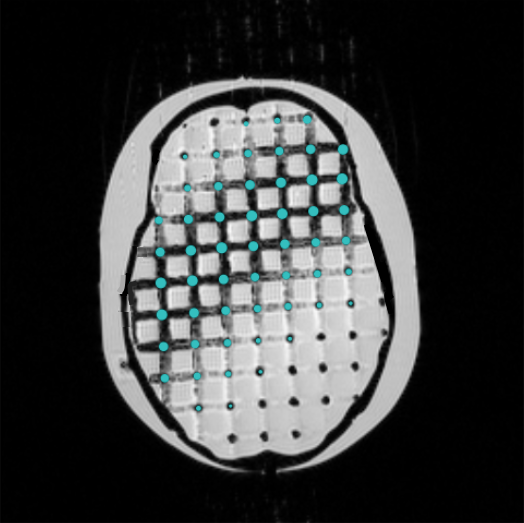
\includegraphics[width=\textwidth]{source-image.png}
        \caption{Source Image}
        \label{fig:test-case_1}
    \end{subfigure}%
    ~
    \begin{subfigure}[b]{0.48\textwidth}
        \centering
        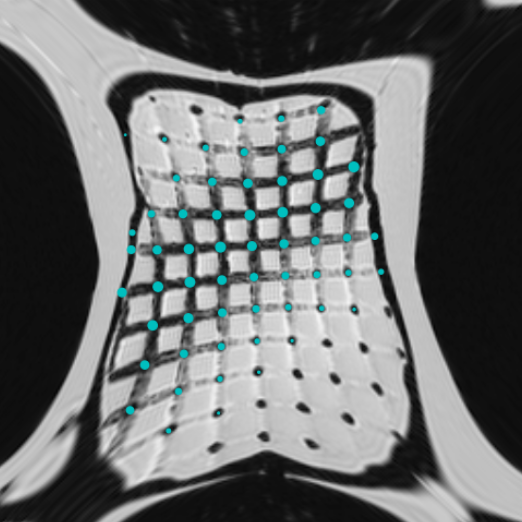
\includegraphics[width=\textwidth]{distorted-image.png}
        \caption{Distorted Image}
        \label{fig:test-case_2}
    \end{subfigure}
    \caption{Example test case with extreme distortion.  In order to validate our algorithms, we apply a known distortion to existing MRI source images.  Fiducials are manually identified on the source image, and are overlaid as light blue circles on the source image, (a).  The size of the circles indicates their position along the slice-axis (i.e. in or out of the page).  The circles overlaid on the distorted image, (b), are the points detected by one of our algorithms for this source image.}
    \label{fig:test-case}
\end{figure}

\subsection{Feature Detection Testing}

Our feature detection test quantifies how well our feature detection stage performs.  It is useful to have a separate test for feature detection because its performance is critical to the performance of the entire algorithm.  Furthermore, although the full system test will demonstrate the existence of errors in the feature detection, the final result will not provide much insight as to why it failed or how to correct the problem.

The feature detection test is very similar to the full system test.  It begins by applying a known distortion to an existing image that has been annotated.  The distorted image is fed into the feature detection algorithm which returns a set of fiducials.  We then want to know if the feature detection detected all of the fiducials it was supposed to, how many superfluous fiducials it detected, and how accurately it located the fiducials.  In particular, we calculate the true positive fraction (k

\begin{figure}
    \centering
    \includegraphics[width=\linewidth]{testing-feature-detection.pdf}
    \caption{Our feature detection test.  Ultimately, the target registration error is the most meaningful metric \cite[page R38]{hill2001}, however, it is useful to understand how well the feature detection stage of the algorithm performed in isolation.  Our feature detection test quantifies what fraction of the fiducials were calculated (the TPF), the number of incorrectly identified fiducials (the FPF), and the mean error of the matched points (the mean FLE).}
    \label{fig:testing-feature-detection}
\end{figure}

\subsection{Visualization Strategies}

\section{Current Algorithm}

Our current algorithm combines our own ideas with those found in the literature (e.g. \cite{stanescu2010,baldwin2007}).  

\subsection{Feature Detection}

Features are detected in the distorted image by convolving it with a 3D kernel shaped like the grid-phantom intersections.  The convolved image tends to have peaks at the feature locations.  We threshold the convolved image and find the center of mass of regions of pixels centered at each peak.

\subsection{Rigid Registration}

At this point, we have a set of automatically calculated fiducials.  Next we need to apply a rigid registration (e.g. Figure \ref{fig:problem-overview}c) so that we can extract the geometric distortion from each pair of matching fiducials.  Performing this rigid registration precisely is complicated by a number of factors.

\section{Discussion}

\bibliographystyle{ieeetr}
\bibliography{./algorithm.bib}

\end{document}
